\chapter{Final Architecture}
\label{chap:final-architecture}

\section{Context Diagram}

\begin{figure}
	\begin{centering}
		% TODO Figure
		%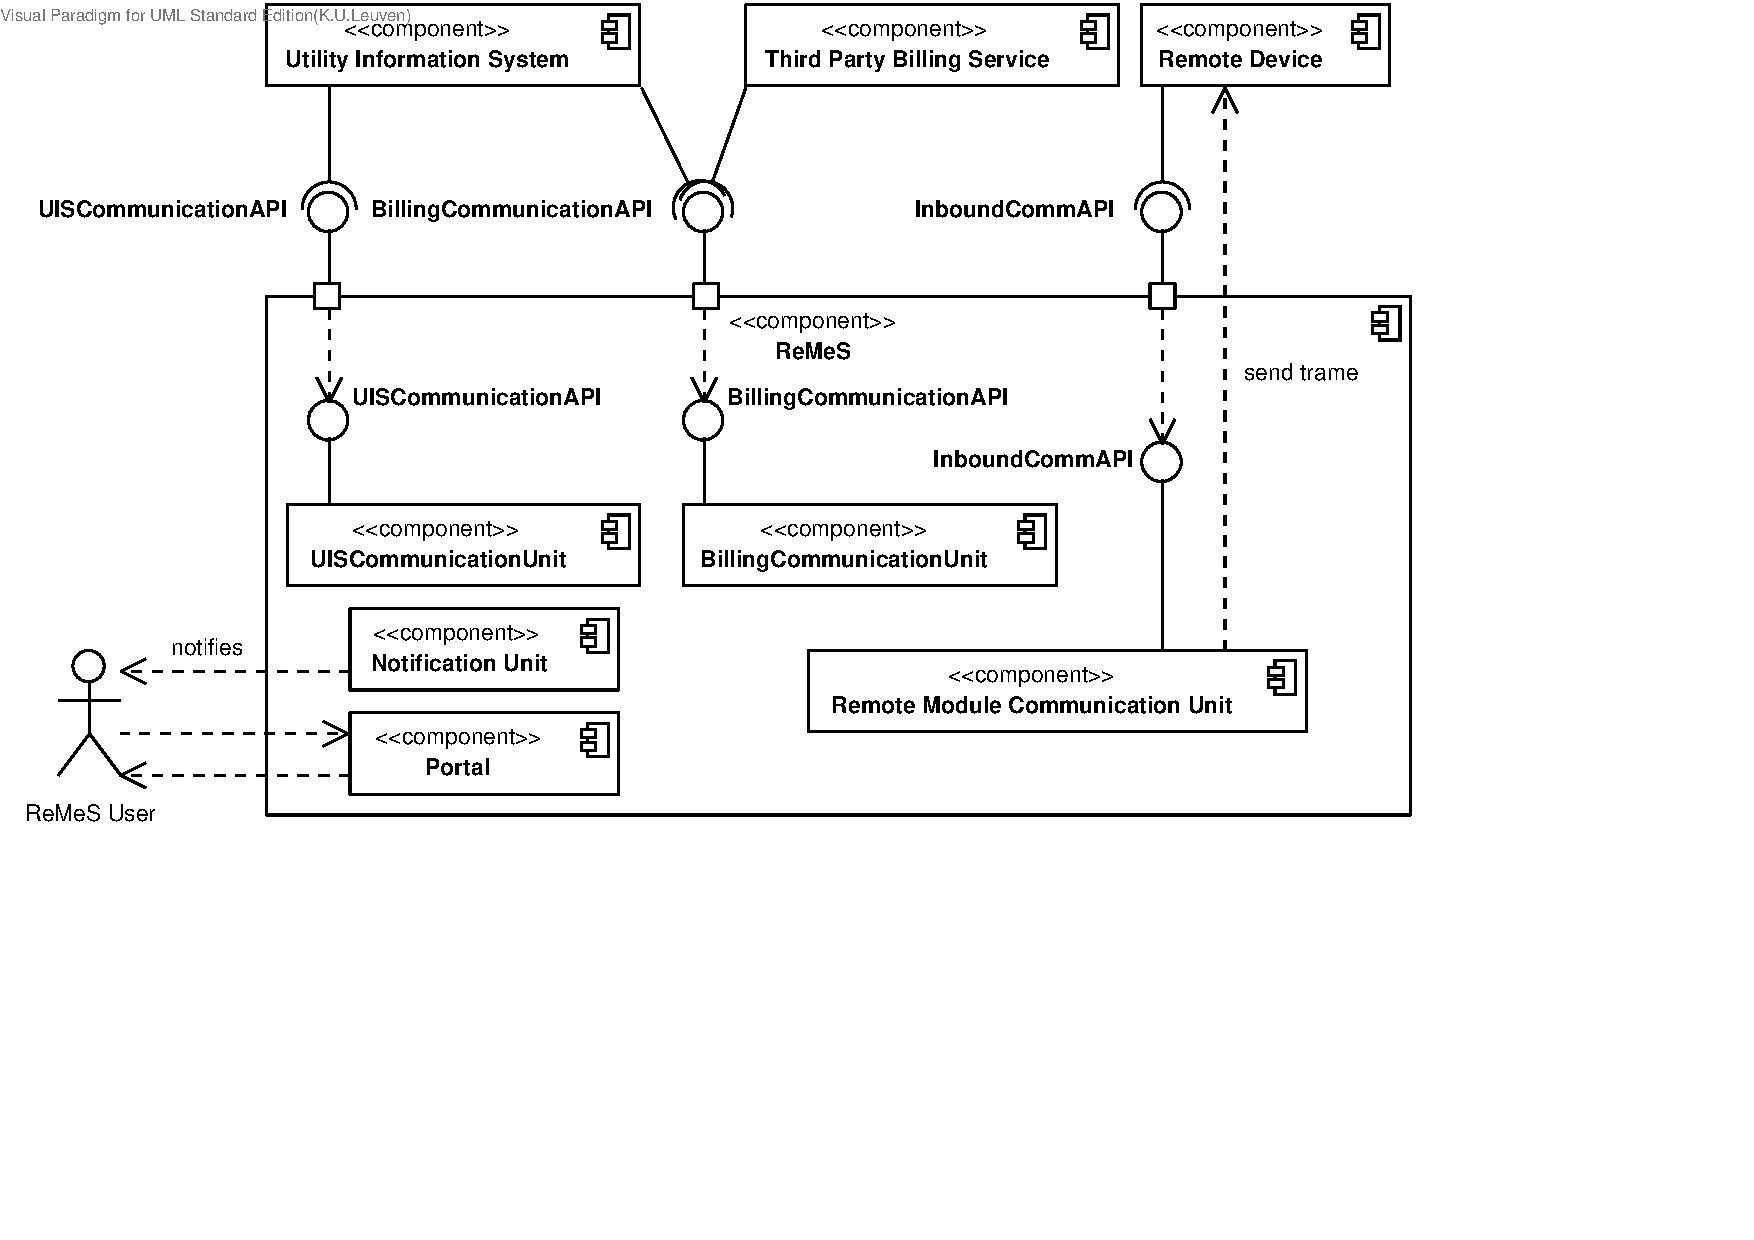
\includegraphics[width=\textwidth]{figs/final-context.pdf}
		\caption{The context diagram}
		\label{fig:final-context}
	\end{centering}
\end{figure}

\npar Figure \ref{fig:final-context} shows the context diagram. The ReMeS
user is a generalisation for all actors who can interact with the portal. 

\section{Overall Component Diagram}

\begin{figure}
	\begin{centering}
		% TODO Figure
		%\includegraphics[width=\textwidth]{figs/final-components.pdf}
		\caption{The component diagram of the overall system}
		\label{fig:final-components}
	\end{centering}
\end{figure}

\section{Key Decompositions}

\section{Deployment Diagram}

\npar The deployment diagram is shown in figure \ref{fig:final-deployment}. 

\begin{figure}
	\begin{centering}
		% TODO Figure
		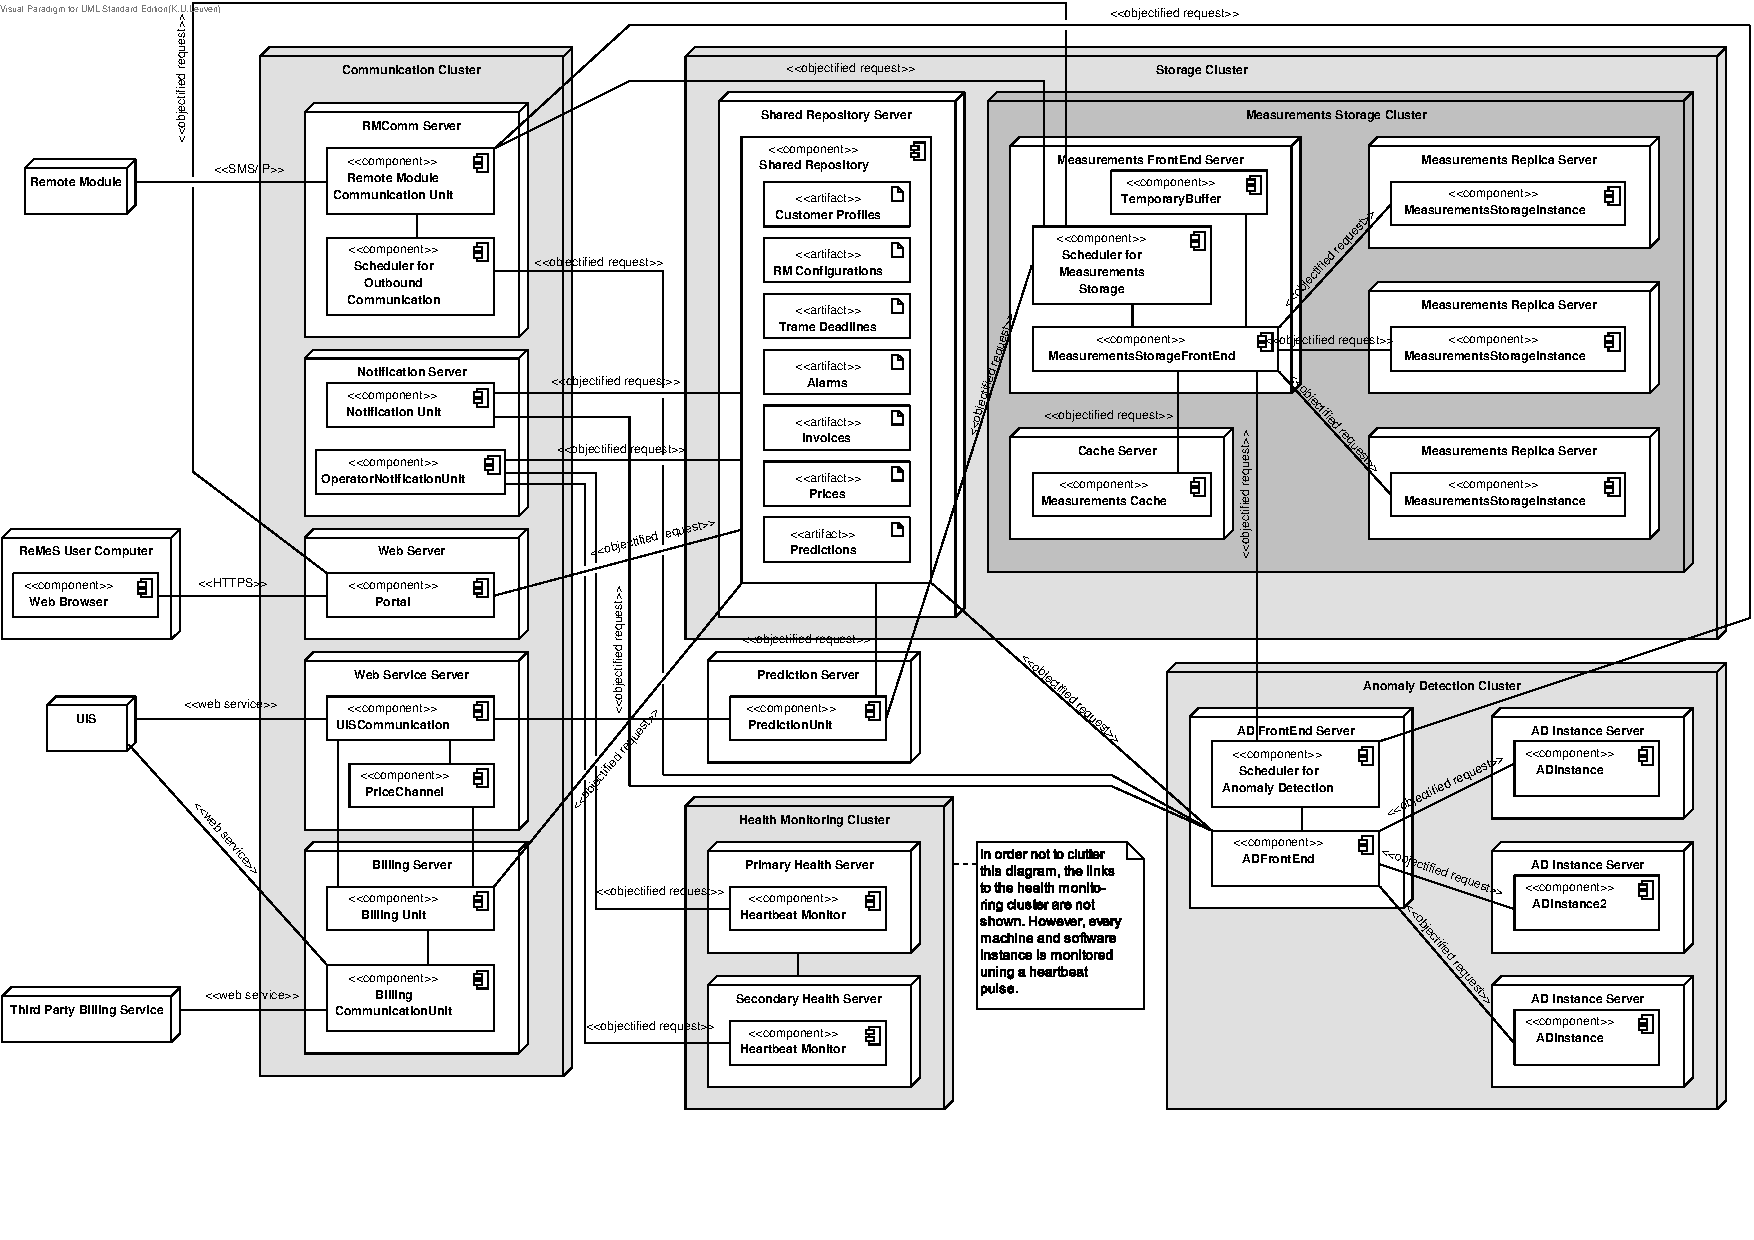
\includegraphics[height=\textwidth,angle=90]{figs/final-deployment.pdf}
		\caption{The deployment diagram}
		\label{fig:final-deployment}
	\end{centering}
\end{figure}

\npar A trame always arrives at the RMComm Server in the Communication Cluster.
This server acts as a gateway for all remote module communication. It will also
host the scheduler for outbound communication. To summarize, the RMComm Server
is responsible for all trame communication. 

\npar As already mentioned, the Communication Unit will route trames to the
right units: a measurement trame is routed to storage, an alarm trame is
immediately routed to the anomaly detection unit. Both units have been assigned
their own clusters: the measurements storage cluster and the anomaly detection
cluster. 

\npar The anomaly detection cluster exists of a frontend server, which takes
care of scheduling, resource arbitration and results processing
(shutting the valve and dispatching the notification unit in case of an alarm).
Among the frontend server, there are a number of anomaly detection instances.
Only three are shown but additional instances can be easily added and/or
removed. This is one of the advantages of the resource pool design pattern.

\npar The measurements storage cluster is contained in a general storage
cluster. Again, as with the anomaly detection cluster, the scheduler, frontend
and buffer are assigned to a single machine. That machine communicates with a
cache server and multiple measurements storage replicas. 

\npar Among the measurements storage cluster, there is a shared repository
server. This machine handles all other storage, from customer profiles to
predictions and historical prices. 

\npar Every machine in the deployment diagram communicates with the heartbeat
cluster. This is, however, not shown in figure \ref{fig:final-deployment}
because it would only make the diagram less clear. This cluster has a primary
server and a secondary server, which monitors the primary and vice versa. This
way, virtually 100\% of both servers can be guaranteed. What is the chance that
both servers fail at exactly the same time?

\npar The notification of ReMeS operators is handled by the Notification Server.
This server is also used to notify alarm recipients and the customer in case of
an alarm. 

\npar The billing is separated from the rest of the system because it is an
expensive operation, happens only once a month and should not affect the
operation of the other systems. 

\npar A similar reasoning is used for the Prediction Server. This is an
expensive operation that should not interfere with the other systems and runs
less often than the other systems.

\npar Communication with the UIS is provided through the Web Service Server. It
is assumed that communication with third parties will be implemented with web
services. 

\npar Last, but not least, a webserver provides access to all ReMeS data. The
traffic between the user's browser and the web server is encypted.

\npar The deployment diagram is created with the idea that is is probably better
to define multiple small, easy replacable machines instead of few, large
do-it-all servers. With the current virtualization technologies, the hardware of
multiple nodes in this system can be shared, which will reduce hardware and
maintenance costs.